
\documentclass[11pt]{article}
\usepackage[margin=0.78in]{geometry}
\usepackage{booktabs}
\usepackage{longtable}
\usepackage{tabularx}
\usepackage{array}
\usepackage{graphicx}
\usepackage{float}
\usepackage{xcolor}
\usepackage{hyperref}
\usepackage{amsmath}
\usepackage{tikz}
\usetikzlibrary{arrows.meta,positioning,shapes.geometric}
\hypersetup{colorlinks=true, linkcolor=blue, urlcolor=blue}
\setlength{\parskip}{0.45em}
\setlength{\parindent}{0pt}
\renewcommand{\arraystretch}{1.13}

\title{TP2 Violation Lifecycle Tracking Report\\\large SPY Call Option Research Pipeline}
\author{ML-Based Trading of TP2-Inspired Violations in SPY American Call Options}
\date{June 22, 2026}

\begin{document}
\maketitle

\section{Purpose}

This report documents the lifecycle layer used before machine learning. The goal is to track each
conservative bid/ask TP2 episode from the pre-violation window through the T1 expiration boundary,
then understand whether the violation is sudden, persistent, tradable, and useful for later
strategy-label construction.

The report reflects the corrected pipeline after the raw-data sanity screen for impossible call
quotes. The clean-data layer now removes call quotes that fail the broad static bound:

\[
\max(S-K,0)-1 \le C_{mid} \le 1.05S+1.
\]

This screen removes raw vendor artifacts such as the March 2017 deep-in-the-money SPY call quote
that was far below intrinsic on one date and above the underlying on another date. It is a data
quality filter, not a Black-Scholes pricing assumption.

\section{Current Pipeline}

\begin{figure}[H]
\centering
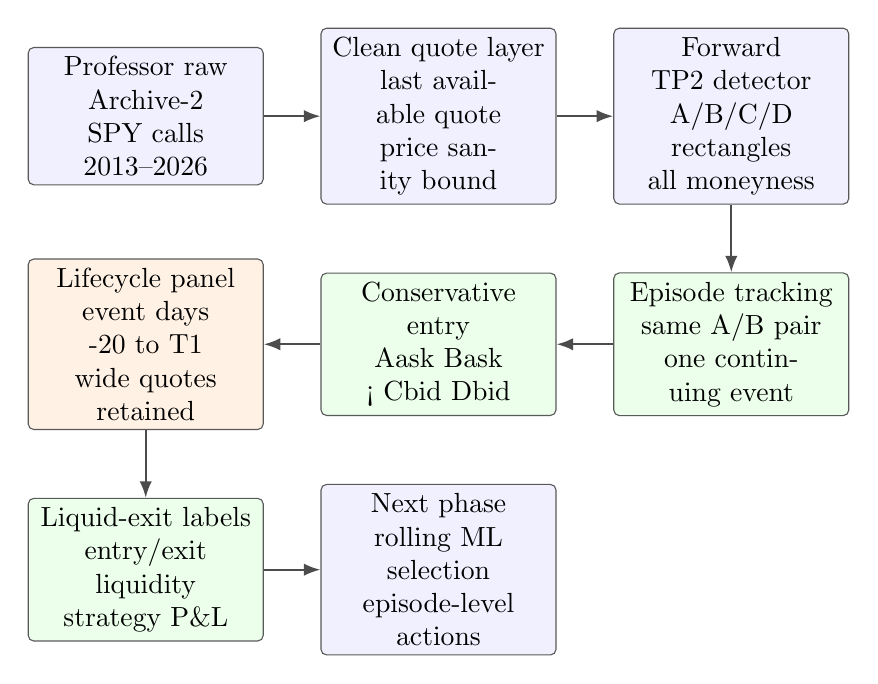
\begin{tikzpicture}[
  node distance=0.86cm and 0.72cm,
  box/.style={rectangle, rounded corners=2pt, draw=black!65, fill=blue!6, text width=2.75cm, align=center, minimum height=0.86cm},
  good/.style={rectangle, rounded corners=2pt, draw=black!65, fill=green!8, text width=2.75cm, align=center, minimum height=0.86cm},
  warn/.style={rectangle, rounded corners=2pt, draw=black!65, fill=orange!10, text width=2.75cm, align=center, minimum height=0.86cm},
  arrow/.style={-{Latex[length=2.1mm]}, thick, draw=black!70}
]
\node[box] (raw) {Professor raw\\Archive-2 SPY calls\\2013--2026};
\node[box, right=of raw] (clean) {Clean quote layer\\last available quote\\price sanity bound};
\node[box, right=of clean] (detect) {Forward TP2 detector\\A/B/C/D rectangles\\all moneyness};
\node[good, below=of detect] (episodes) {Episode tracking\\same A/B pair\\one continuing event};
\node[good, left=of episodes] (conservative) {Conservative entry\\Aask Bask < Cbid Dbid};
\node[warn, left=of conservative] (lifecycle) {Lifecycle panel\\event days -20 to T1\\wide quotes retained};
\node[good, below=of lifecycle] (exit) {Liquid-exit labels\\entry/exit liquidity\\strategy P\&L};
\node[box, right=of exit] (ml) {Next phase\\rolling ML selection\\episode-level actions};
\draw[arrow] (raw) -- (clean);
\draw[arrow] (clean) -- (detect);
\draw[arrow] (detect) -- (episodes);
\draw[arrow] (episodes) -- (conservative);
\draw[arrow] (conservative) -- (lifecycle);
\draw[arrow] (lifecycle) -- (exit);
\draw[arrow] (exit) -- (ml);
\end{tikzpicture}
\caption{Final pre-ML pipeline. The lifecycle report covers the highlighted lifecycle layer and its connection to liquid-exit labels.}
\end{figure}

\section{Core Counts}

\begin{center}
\begin{tabular}{lr}
\toprule
Quantity & Value \\
\midrule
Raw rows & 58,834,075 \\
Deduplicated rows & 22,589,850 \\
Clean call rows & 4,910,706 \\
Daily TP2 violation rows & 2,419,378 \\
Pair episodes & 2,091,823 \\
Conservative bid/ask entry episodes & 226,577 \\
Lifecycle rows & 6,356,278 \\
Lifecycle event-day range & -20 to 53 \\
Observable lifecycle rows & 2,364,764 \\
Conservative bid/ask lifecycle violation rows & 364,024 \\
\bottomrule
\end{tabular}
\end{center}

\section{Lifecycle Definition}

Event day 0 is the first conservative bid/ask TP2 violation date for an episode. Negative event
days are pre-violation observations of the same left-side pair; positive event days track the same
economic pair forward until T1 expiration. On each lifecycle date, the pipeline reconstructs the
right-side C/D legs using the current forward-adjusted round-up rule.

Normalized pressure is:

\[
\text{pressure} = \frac{C_{mid}D_{mid} - A_{mid}B_{mid}}{C_{mid}D_{mid} + A_{mid}B_{mid}}.
\]

Positive pressure means a mid-price TP2 violation. Conservative bid/ask violation is stricter:

\[
A_{ask}B_{ask} < C_{bid}D_{bid}.
\]

Wide-spread rows are kept for behavior tracking, but they are not executable trade exits unless
the selected legs pass the liquidity rule at the entry/exit point.

\section{Event-Time Summary}

\begin{center}
\resizebox{\linewidth}{!}{%
\begin{tabular}{rrrrrrrrr}
\toprule
Day & Episodes & Evaluable & Median pressure & P25 & P75 & Mid violation & Bid/ask violation & All legs liquid \\
\midrule
-20 & 226,577 & 40,798 & -0.0788 & -0.2060 & -0.0291 & 0.78\% & 0.42\% & 17.63\% \\
-10 & 226,577 & 71,692 & -0.0711 & -0.2230 & -0.0136 & 6.49\% & 5.24\% & 30.08\% \\
-5 & 226,577 & 103,311 & -0.0588 & -0.2561 & 0.0191 & 12.96\% & 9.99\% & 42.44\% \\
-1 & 226,577 & 141,862 & -0.1023 & -0.3605 & -0.0327 & 6.65\% & 1.58\% & 50.67\% \\
0 & 226,577 & 226,577 & 0.1928 & 0.0542 & 0.2802 & 100.00\% & 100.00\% & 100.00\% \\
1 & 188,077 & 110,656 & -0.0546 & -0.3267 & 0.0039 & 14.98\% & 4.65\% & 40.73\% \\
3 & 156,810 & 78,940 & -0.0577 & -0.2201 & -0.0144 & 10.41\% & 3.78\% & 38.25\% \\
5 & 128,809 & 58,525 & -0.0503 & -0.1628 & -0.0071 & 10.88\% & 6.60\% & 37.89\% \\
10 & 59,142 & 32,921 & -0.0672 & -0.2126 & -0.0164 & 9.13\% & 5.32\% & 47.32\% \\
20 & 16,982 & 7,871 & -0.0651 & -0.3171 & -0.0163 & 2.00\% & 1.25\% & 44.24\% \\
40 & 889 & 473 & -0.0687 & -0.1605 & -0.0440 & 0.00\% & 0.00\% & 53.21\% \\
53 & 15 & 0 & NA & NA & NA & 0.00\% & 0.00\% & 0.00\% \\
\bottomrule
\end{tabular}
}
\end{center}

Interpretation: the violation begins at day 0 by construction, but the pre-event rows show whether
the same pair was already near the TP2 boundary. Fast decay after day 0 supports reversion-style
labels; persistent positive pressure indicates a harder trade because the dislocation does not
correct quickly.


\begin{figure}[H]
  \centering
  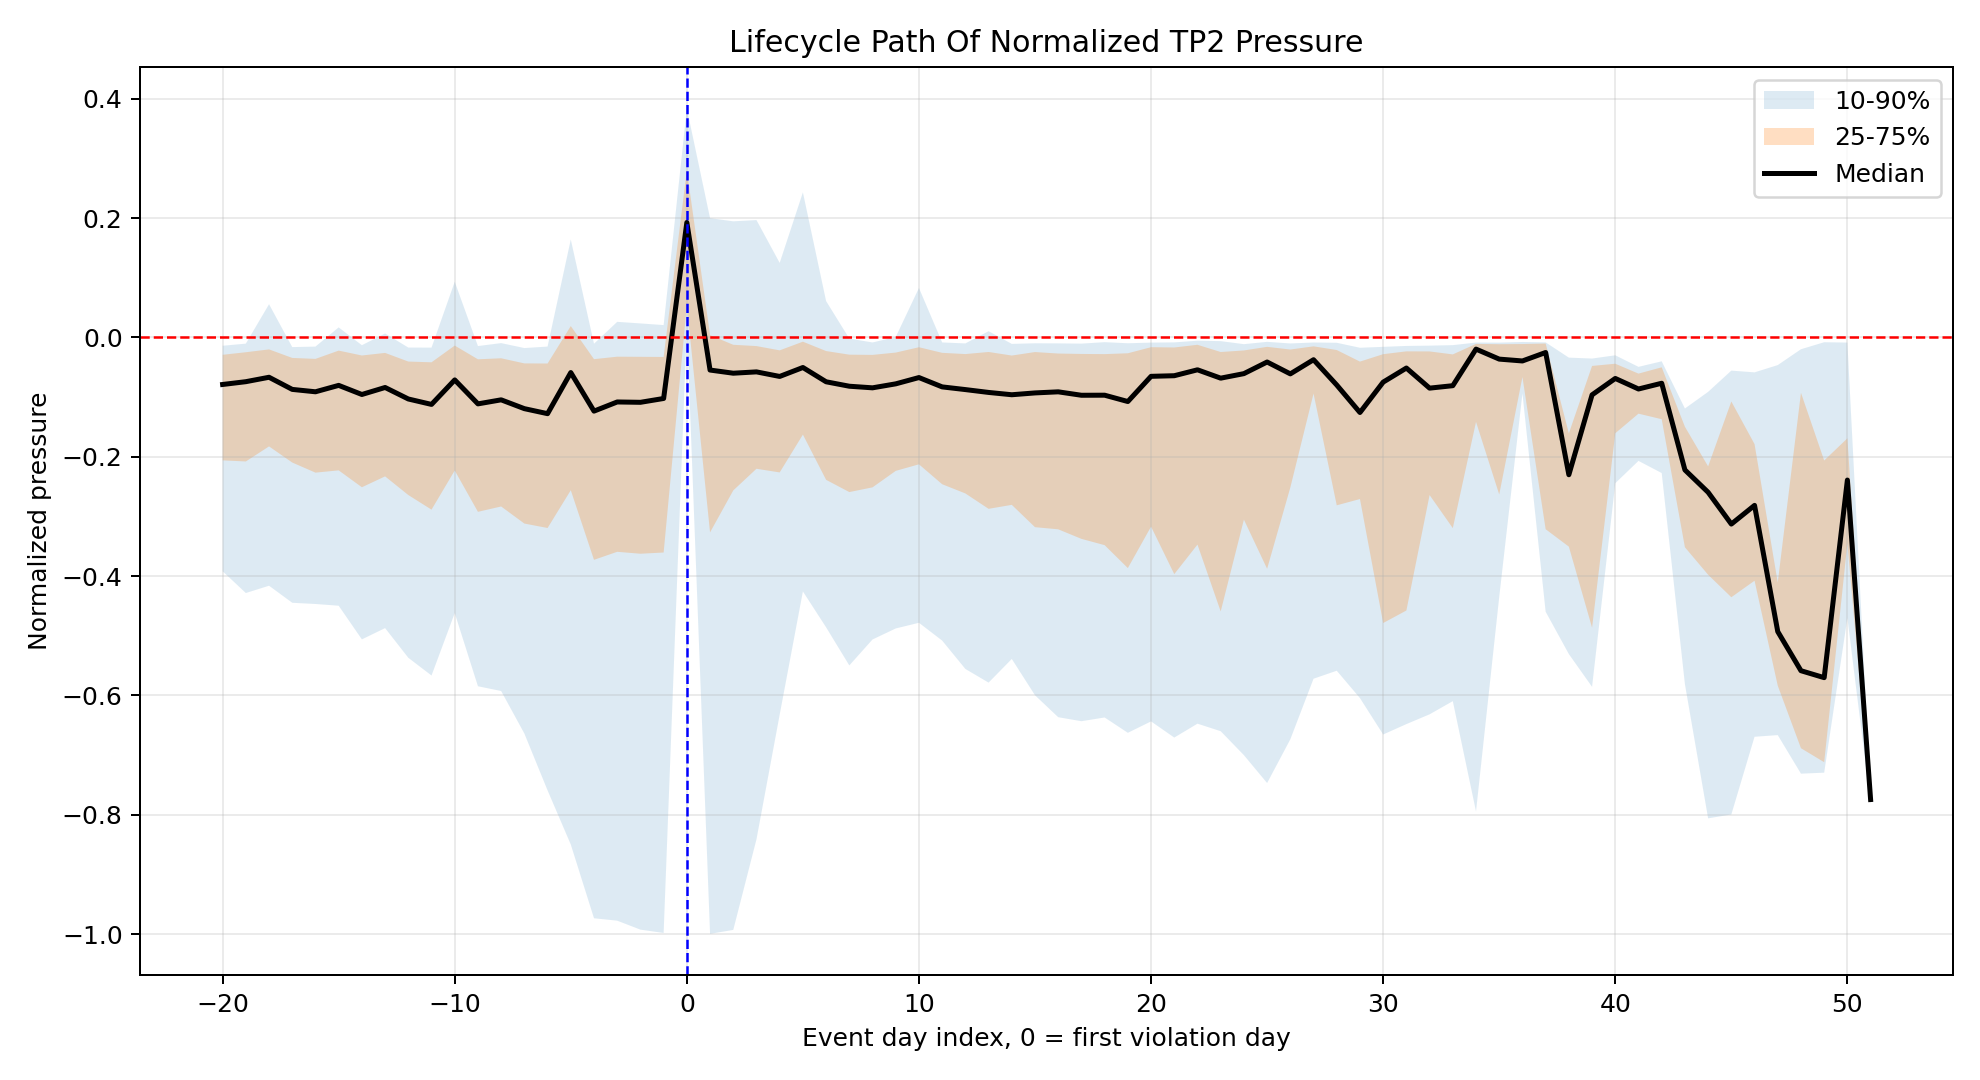
\includegraphics[width=0.92\linewidth]{figures/lifecycle_normalized_pressure_band.png}
  \caption{Median normalized pressure with 25--75 and 10--90 percentile bands. The dashed vertical line is the first violation day.}
  \label{fig:lifecycle-pressure-band}
\end{figure}



\begin{figure}[H]
  \centering
  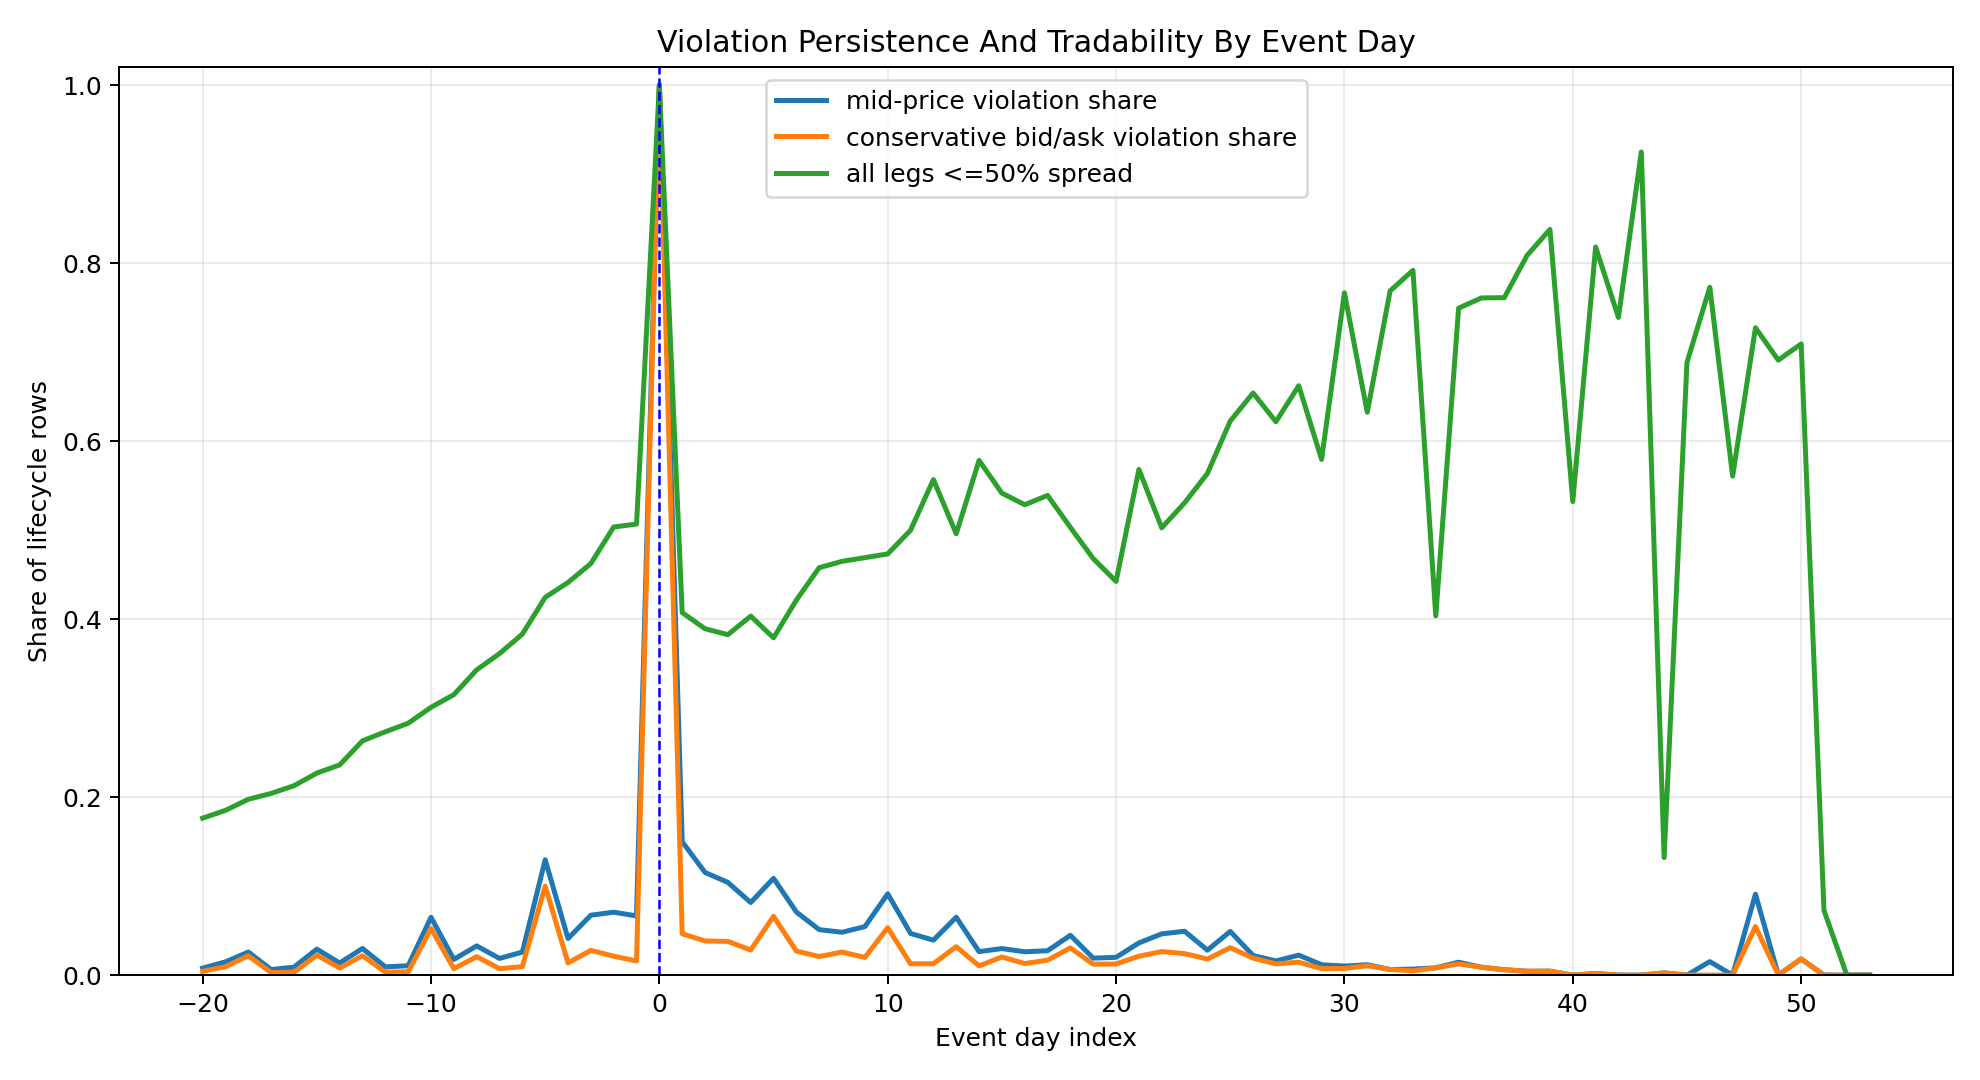
\includegraphics[width=0.92\linewidth]{figures/lifecycle_violation_tradability_share.png}
  \caption{Share of lifecycle rows that remain mid-price violations, conservative bid/ask violations, and all-leg liquid under the 50\% spread rule.}
  \label{fig:lifecycle-tradability}
\end{figure}


\section{Status And Observability}

\begin{center}
\resizebox{0.98\linewidth}{!}{%
\begin{tabular}{rrrrrr}
\toprule
Day & Observable & Wide spread & Missing A/B & Missing C/D & Missing F \\
\midrule
-20 & 17.63\% & 0.38\% & 78.09\% & 0.18\% & 3.69\% \\
-10 & 30.08\% & 1.56\% & 62.35\% & 0.46\% & 5.50\% \\
-5 & 42.44\% & 3.16\% & 49.76\% & 1.06\% & 3.51\% \\
-1 & 50.67\% & 11.94\% & 34.73\% & 2.25\% & 0.19\% \\
0 & 100.00\% & 0.00\% & 0.00\% & 0.00\% & 0.00\% \\
1 & 40.73\% & 18.11\% & 35.44\% & 4.19\% & 1.37\% \\
3 & 38.25\% & 12.09\% & 37.13\% & 10.80\% & 1.54\% \\
5 & 37.89\% & 7.54\% & 40.29\% & 12.57\% & 1.46\% \\
10 & 47.32\% & 8.35\% & 32.81\% & 10.69\% & 0.58\% \\
20 & 44.24\% & 2.11\% & 46.40\% & 6.78\% & 0.25\% \\
40 & 53.21\% & 0.00\% & 45.89\% & 0.00\% & 0.90\% \\
53 & 0.00\% & 0.00\% & 100.00\% & 0.00\% & 0.00\% \\
\bottomrule
\end{tabular}
}
\end{center}

Observable means all reconstructed A/B/C/D legs and forward inputs are available on that lifecycle
date. Missing A/B usually appears in pre-violation lookback when one of the left-pair contracts was
not listed yet. Missing C/D means the forward-adjusted right leg could not be reconstructed on that
date. Wide spread means the rectangle is observable but at least one leg fails the 50\% spread
liquidity rule.


\begin{figure}[H]
  \centering
  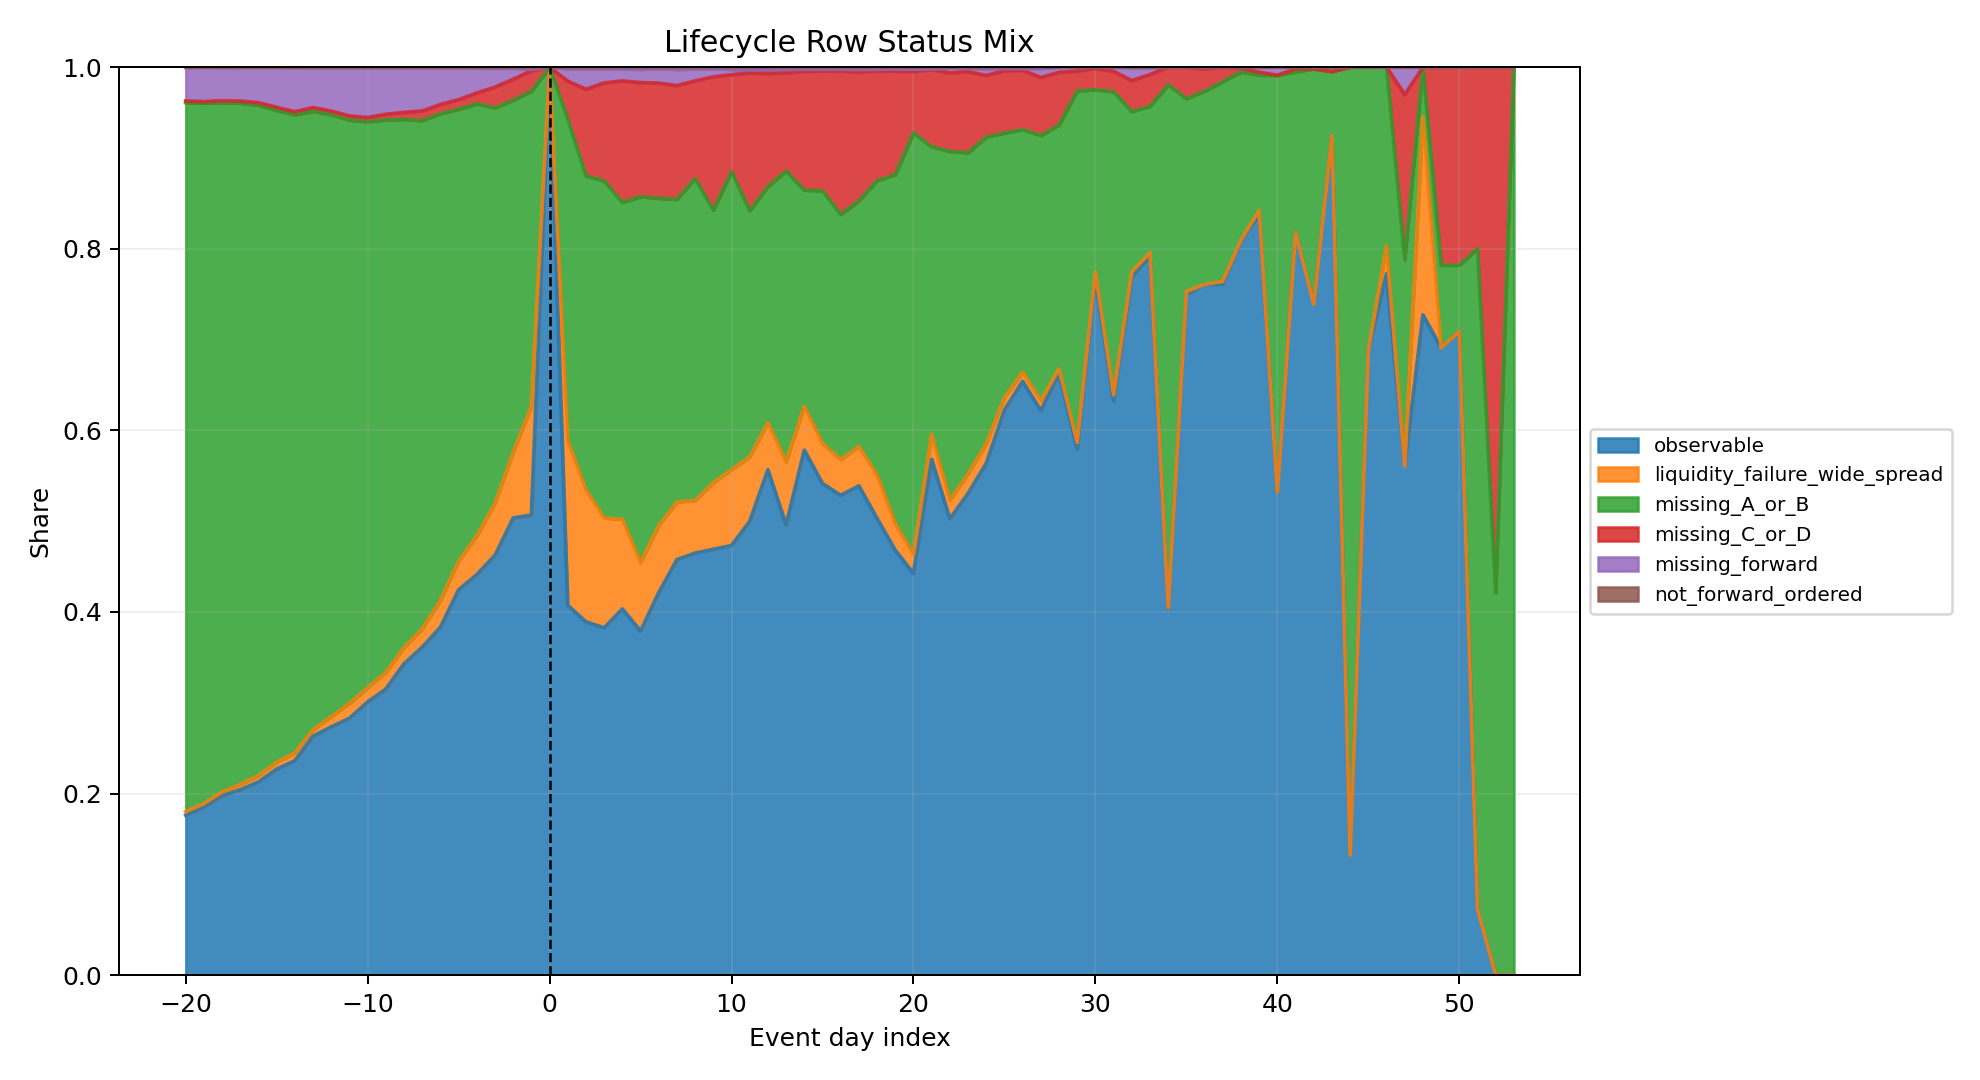
\includegraphics[width=0.92\linewidth]{figures/lifecycle_status_mix_by_event_day.png}
  \caption{Lifecycle row status mix by event day. This separates economic non-reversion from quote/contract availability.}
  \label{fig:lifecycle-status}
\end{figure}


\section{Outcome Split}

The lifecycle path is not itself a live trading label, but it helps diagnose whether entry-time
features might predict profitable exits. The next figure splits median pressure paths by T1
product-weighted outcome. Only event days at or before 0 can become ML features; future paths are
used for labels and diagnostics only.


\begin{figure}[H]
  \centering
  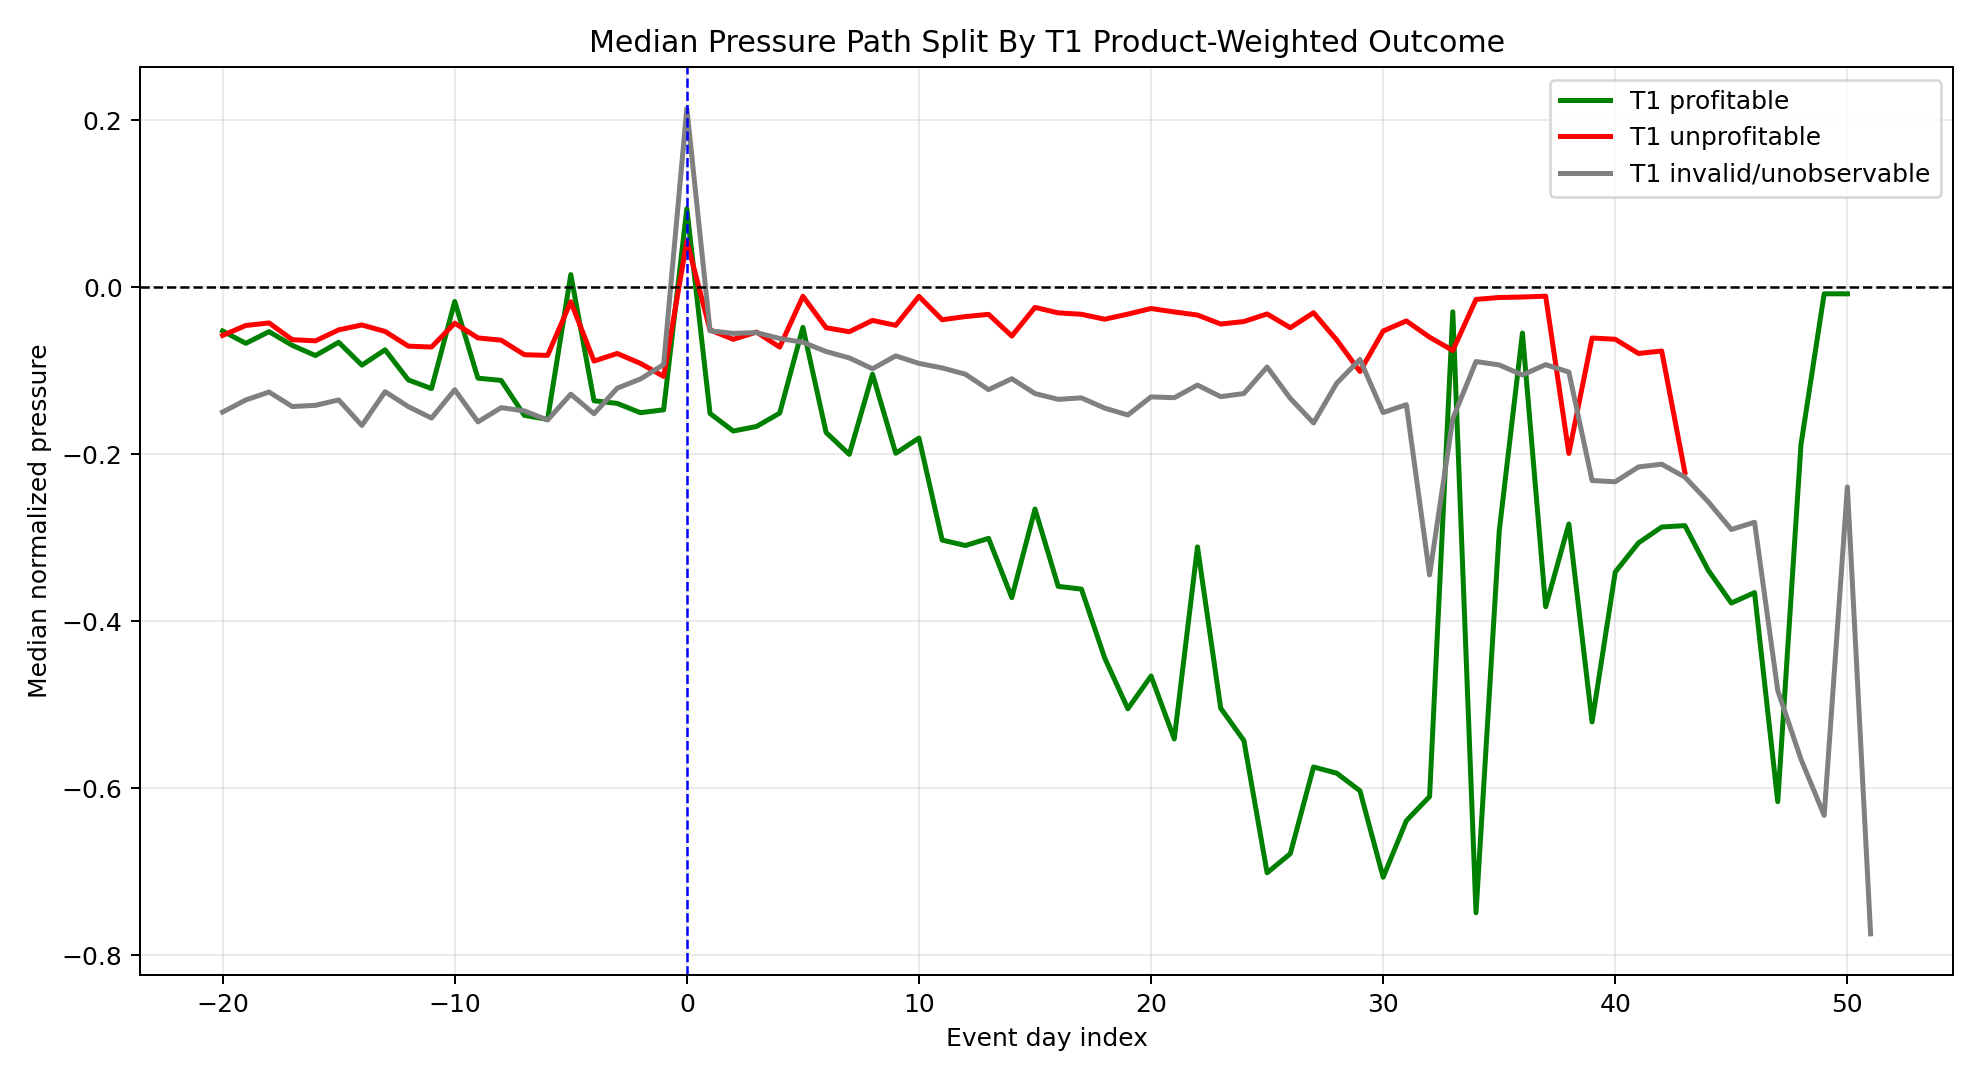
\includegraphics[width=0.92\linewidth]{figures/lifecycle_pressure_by_T1_outcome.png}
  \caption{Median pressure path split by T1 product-weighted backtest outcome.}
  \label{fig:lifecycle-outcome}
\end{figure}



\begin{figure}[H]
  \centering
  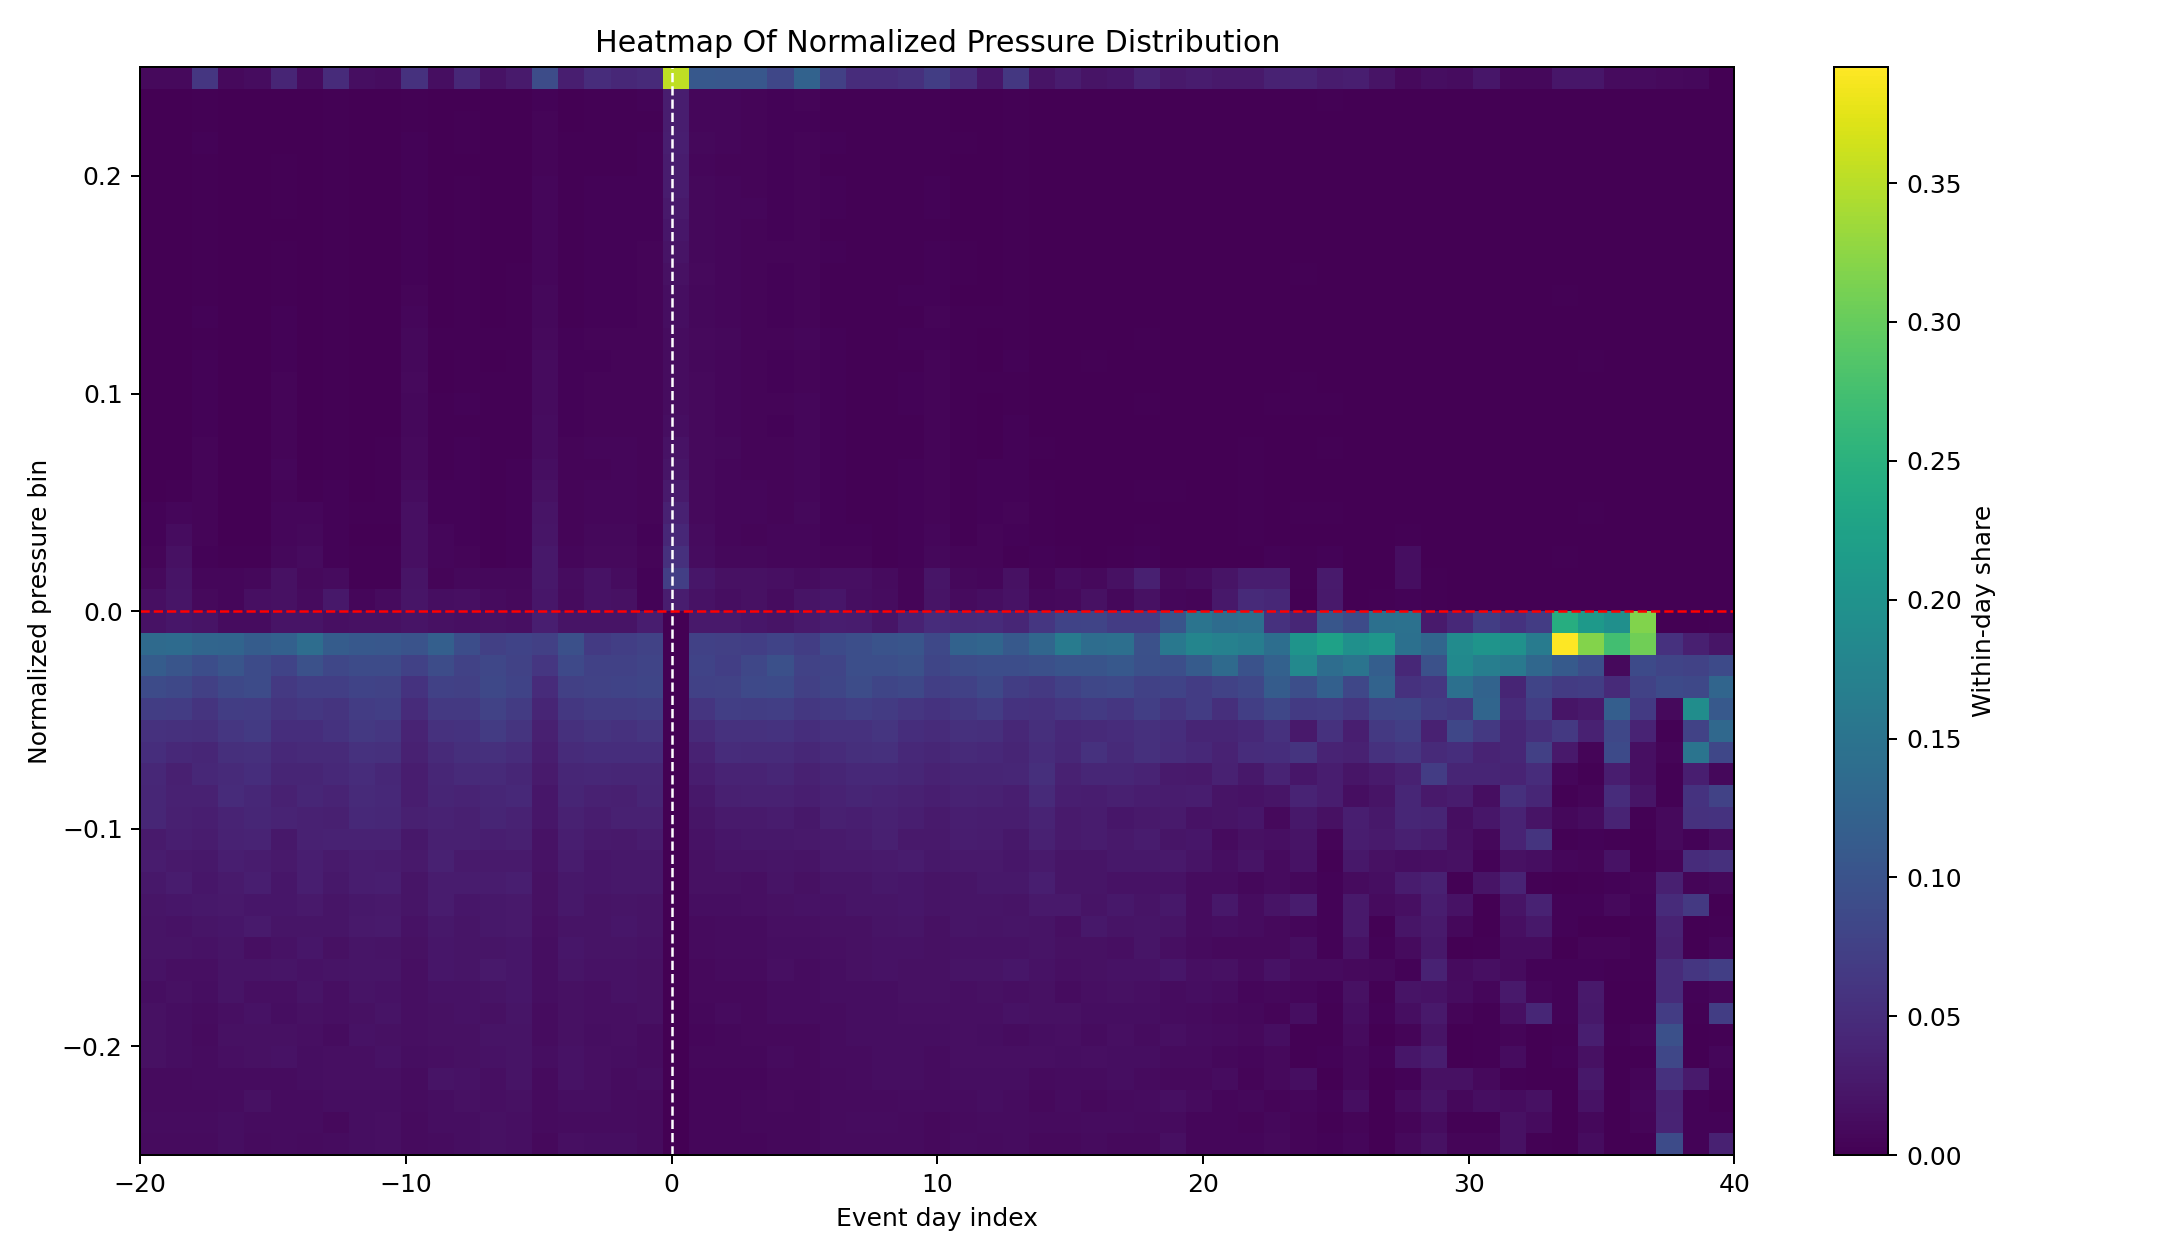
\includegraphics[width=0.92\linewidth]{figures/lifecycle_pressure_heatmap.png}
  \caption{Distribution of normalized pressure by event day. This shows concentration near zero versus extreme dislocations.}
  \label{fig:lifecycle-heatmap}
\end{figure}


\section{Data Quality Correction}

\begin{center}
\begin{tabular}{rrr}
\toprule
Year & Clean rows & Sanity-filtered rows \\
\midrule
2014 & 156,422 & 57 \\
2017 & 242,021 & 20 \\
2018 & 340,878 & 26 \\
2020 & 527,851 & 232 \\
2021 & 567,866 & 68 \\
2022 & 539,279 & 203 \\
2023 & 410,307 & 3 \\
2024 & 483,637 & 21 \\
2025 & 522,372 & 1,532 \\
2026 & 258,565 & 23 \\
\bottomrule
\end{tabular}
\end{center}

These are otherwise eligible clean-layer rows removed by the call-price sanity bound. The 2017
artifact that created the previous abnormal P\&L spike is removed here; the corrected liquid-exit
labels contain zero rows involving that bad contract in the strategy legs.

\section{What Is Left Before ML}

\begin{enumerate}
\item Lock the target definition: choose whether the first ML target is T1/K1 first-liquid P\&L,
positive return classification, or a three-way action label of skip/T1/K1.
\item Build only point-in-time features: signal-date surface features, bid/ask severity,
moneyness, DTE gaps, liquidity flags, prior pressure path summaries from event days \(\le 0\),
and no future lifecycle columns.
\item Add concentration controls: report results with winsorized P\&L, capped position size, and
top-episode contribution so one date cannot dominate conference results.
\item Define rolling evaluation: train on past years, validate on the next block, test on the
following block, then roll forward. No random row split.
\item Add transaction-cost and execution assumptions: keep bid/ask fills, contract multiplier,
and option fee assumptions in the labels and report both gross and net performance.
\end{enumerate}

\section{Conclusion}

The pre-ML pipeline is now conceptually ready for model construction. The major remaining work is
not more cleaning; it is label choice, leakage-proof feature construction, rolling evaluation, and
robustness reporting. The lifecycle layer provides the key bridge: it tells us how violations
behave before and after first detection while preserving a clear separation between observable
history, future labels, and executable liquidity.

\end{document}
